\vspace{1cm}
\fancyhead[C]{\normalsize\textbf{$\qquad$ Teil I: Offene Aufgaben}}
\renewcommand{\labelenumi}{\theenumi.}
\section*{Aufgabe 1 (40 Punkte)}
\vspace{0.4cm}
\subsection*{\aufgabe{a}{14}}
Das Newton'sche Abkühlungsgesetz beschreibt, wie sich die Temperatur eines Körpers, der sich in einem Raum mit konstanter Temperatur $ T $ befindet, mit der Zeit verändert (das Gesetz beschreibt Abkühlung und Erwärmung gleichermassen).
Im Detail besagt das Abkühlungsgesetz, dass die Änderung der Temperatur eines Körpers zwischen Zeitpunkt $ k $ und $ k+1 $ proportional zur Differenz zwischen der Temperatur des abkühlenden Körpers zum Zeitpunkt $ k $ und der Umgebungstemperatur $ T $ ist. Die Proportionalitätskonstante hängt von der Beschaffenheit des Körpers ab und sei durch den Parameter $ \lambda \in \mathbb{R} \setminus \{0\} $ bestimmt.
\begin{enumerate}
	\item[\textbf{(a1)}]
	Die Temperatur des Körpers zum Zeitpunkt $ k $ sei $ y_k $.
	Leiten Sie eine Differenzengleichung her, die die Entwicklung der Temperatur $ y_k $ für $ k = 1,2,... $ abhängig von der anfänglichen Temperatur $ y_0 $ und der Raumtemperatur $ T  $ beschreibt.
	\item[\textbf{(a2)}] 
	Finden Sie die allgemeine Lösung der Differenzengleichung aus \textbf{(a1)}.
	\item[\textbf{(a3)}] 
	Für welche Werte $ \lambda $ sinkt die Temperatur des Objekts auf lange Sicht (d.h., für $ k \to \infty $) unter 30 ($ ^\circ $C), dass $ y_0 = 100 $ ($ ^\circ $C) und $ T= 20 $ ($ ^\circ $C)?
	Welche dieser Werte wiederum sind auch physikalisch plausibel?
	\item[\textbf{(a4)}]
	Sei $ y_0 = 30  $ ($ ^\circ  $C) und $ T = 15 $ ($ ^\circ  $C).
	Bestimmen Sie den Parameter $ \lambda $ so, dass die Temperatur
	des Körpers zum Zeitpunkt $ k= 10 $ noch $ 16.6 $ ($ ^\circ  $C) beträgt.
	Runden Sie auf eine Dezimalstelle. Wie viel Zeit vergeht, bis $ y_k $ wieder über $ 20 $ ($ ^\circ  $C) steigt, wenn zum Zeitpunkt $ k = 10 $ die Raumtemperatur auf $ T = 25 $ ($ ^\circ  $C) erhöht wird?
\end{enumerate}
\ \\

\textbf{Lösung:}
\begin{mdframed}
\underline{\textbf{Vorgehensweise:}}
\renewcommand{\labelenumi}{\theenumi.}
\begin{enumerate}
\item[\textbf{(a1)}]
\begin{enumerate}
	\item[1.] Stelle die Differenzengleichung auf.
	\item[2.] Forme in die Normalform um.
\end{enumerate} 
\item[\textbf{(a2)}]
\begin{enumerate}
	\item[1.] Bestimme die Lösungen mithilfe der Normalform.
\end{enumerate} 
\item[\textbf{(a3)}]
\begin{enumerate}
	\item[1.] Unterscheide geeignete Fälle anhand der Normalform.
\end{enumerate}
\item[\textbf{(a4)}]
\begin{enumerate}
	\item[1.] Bestimme den Parameter $ \lambda $.
	\item[2.] Stelle eine neue Differenzengleichung für das veränderte Problem auf.
\end{enumerate}  
\end{enumerate}
\end{mdframed}
\underline{(\textbf{a1}) 1. Stelle die Differenzengleichung auf}\\
Sei $ y_k $ die Temperatur des Körpers zu dem Zeitpunkt $ k $.
Die Änderung der Temperatur des Körpers zwischen dem Zeitpunkt $ k $ und $ k+1 $ ist gegeben durch $ y_{k+1} - y_k $.
Die Differenz des Körpers zum Zeitpunkt $ k $ und der Umgebungstemperatur $ T $ wird durch $ y_k - T $ ausgedrückt.
Das Newton'sche Abkühlungsgesetz besagt, dass die Temperaturänderung proportional zur Differenz des Körpers zum Zeitpunkt $ k $ und der Umgebungstemperatur $ T $ des Raumes ist.
Formal bedeutet dies
\begin{align*}
	\frac{y_{k+1}- y_k}{y_k - T} = \lambda
	\ \Leftrightarrow \
	y_{k+1} - y_k = \lambda \cdot (y_k - T), \quad k = 0,1,2,...
\end{align*}
für die Proportionalitätskonstante $ \lambda \in \mathbb{R} \setminus \{0\} $.
Damit liegt eine lineare Differenzengleichung erster Ordnung mit konstanten Koeffizienten vor.\\
\\
\underline{(\textbf{a1}) 2. Forme in die Normalform um}\\
Eine lineare Differenzengleichung erster Ordnung mit konstanten Koeffizienten lässt sich in die Normalform
\begin{align*}
	y_{k+1} = A y_k + B
\end{align*}
mit $ A, B \in \mathbb{R} $ und $ A \neq  0$ umformen. 
Für das Newton'sche Abkühlungsgesetz bedeutet dies
\begin{align*}
	y_{k+1} - y_k = \lambda \cdot (y_k - T)
	\ \Leftrightarrow \
	y_{k+1} = \lambda \cdot (y_k - T) + y_k
	= \lambda y_k - \lambda T + y_k
	=(\lambda + 1) y_k - \lambda T
\end{align*}
für $ k = 0,1,2,.. $.
In der Notation der Normalform bedeutet dies $ A = \lambda + 1 , \lambda \neq -1 $ und $ B = - \lambda T $.\\
\\
\underline{\textbf{(a2)} 1. Bestimme die Lösungen mithilfe der Normalform}\\
Wenn die Normalform
\begin{align*}
	y_{k+1} = A y_k + B, \quad k = 0,1,2,...
\end{align*}
vorliegt, ist die allgemeine Lösung abhängig von $ A $. Formal drückt sich dies aus in:
\begin{align*}
	y_k = 
	\begin{cases}
		A^k(y_0 - y^\star) 	+y^\star&, \ \text{falls} \ A \neq 1\\
		y_0 + k \cdot B      &, \ \text{falls} \ A = 1 
	\end{cases}
	\quad
	\ \text{mit} \
	y^\star = \frac{B}{1-A}.
\end{align*}
In unserer Aufgabe ist $ A = \lambda + 1  $, womit wir die Fälle $ \lambda = 0  $ und $ \lambda \neq 0  $ unterscheiden müssen.
Für $ \lambda = 0 $ ergibt sich wegen $ B = -\lambda T $ die allgemeine Lösung:
\begin{align*}
	y_k = y_0 ,\quad k= 0,1,2,... \ .
\end{align*}
Für $ \lambda \neq 0 $ erhalten wir mit $ y^\star =
\frac{B}{1- A} = \frac{-\lambda T}{1 - (1+ \lambda)} = \frac{-\lambda T}{-\lambda}
= T $:
\begin{align*}
	y_k = A^k(y_0 - y^\star) 	+y^\star
	=
	(1+ \lambda)^k (y_0 - T) + T.
\end{align*}
Insgesamt erhalten wir die allgemeine Lösung:
\begin{align*}
		y_k = 
	\begin{cases}
		(1+ \lambda)^k (y_0 - T) + T&, \ \text{falls} \ \lambda \neq 0\\
		y_0 &, \ \text{falls} \ \lambda = 0
	\end{cases}.
\end{align*}
\ \\
\underline{\textbf{(a3)} 1. Unterscheide geeignete Fälle anhand der Normalform}\\
Der Fall $ \lambda = 0  $ ist ausgeschlossen, da ansonsten dauerhaft $ y_k = y_0  = 100 $ gilt. 
Wegen $ y_0 - T = 100 - 20 = 80 $ ist $ (y_0 - T) > 0 $. 
Für $ | A | = |1+ \lambda | > 1 $ ist die Folge divergent. Dies ist physikalisch  nicht sinnvoll, denn für $ A > 1 $ gilt $ |y_k| \to \infty $.
Nun bleibt noch $ |A| = |1+ \lambda| < 1 $ übrig. Hierfür gilt:
\begin{align*}
	|1+ \lambda| < 1
	\ \Leftrightarrow \
	-1 < 1 + \lambda < 1
	\ \Leftrightarrow \
	-2 < \lambda < 0.
\end{align*}
Wir wissen also , dass $ y_k $ für $ \lambda \in (-2,0) $ gegen $ y^\star = T = 20 $ ($ ^\circ  $C) konvergiert. Damit fällt die Temperatur für $\lambda \in (-2,0)$ auf lange Sicht unter $ 30 $ ($ ^\circ  $C).
Jedoch ist die Lösung für \\
$ \lambda \in (-2,-1) \subset (-2,0)  $ physikalisch nicht plausibel, da dann $ -1 < A = 1+ \lambda <0 $ gilt und die Lösung oszilliert.
Formal sieht man dies zum Beispiel an:
\begin{align*}
	y_1 = A^1 (y_0 - T) + T
	= 
	\underbrace{A (y_0 - T ) + T}_{< T}.
\end{align*}
Das würde bedeuten, dass ie Temperatur zum Zeitpunkt $ 1 $ kleiner als die Raumtemperatur $ T $, obwohl die Temperatur zum Zeitpunkt $ 0 $ $ 100 $ ($ ^\circ  $C) beträgt.
Für $ \lambda \in (-1,0) $ gilt $ 0 < A < 1 $, womit die Lösung streng monoton fällt und gegen $ y^\star = 20  $ konvergiert.
Insgesamt können wir sagen, dass die Temperatur genau dann auf lange Sicht (physikalisch sinnvoll) unter $ 30 $ ($ ^\circ  $C) fällt, wenn $ \lambda \in (-1,0) $ gilt.\\
\\
\underline{\textbf{(a4)} 1. Bestimme den Parameter $ \lambda $}\\
Gegeben sind $ y_0 = 30  $, $ y_{10} = 16.6 $ und $ T = 15 $.
Gesucht ist das zugehörige $ \lambda $ für das Abkühlungsgesetz.
Dies erhalten wir durch:
\begin{align*}
	&16.6 = y_{10} = (1+ \lambda)^{10} ( y_0 - T) + T
	=
	(1+ \lambda)^{10} (30 - 15) + 15
	=
	(1+ \lambda )^{10} \cdot 15 + 15\\
	\ \Leftrightarrow \
	&\frac{16.6 - 15}{15} = (1+ \lambda )^{10}\\ 
	\ \Leftrightarrow \
	&1+ \lambda= \sqrt[10]{\frac{1.6}{15}}\\
	\ \Leftrightarrow \
	&\lambda = 
	\sqrt[10]{\frac{1.6}{15}} -1 
	\approx 
	-0.2.
\end{align*}
Da die Propornalitätskonstante $ \lambda $ nur von dem Körper abhängt, wird diese durch Änderung der Umgebungstemperatur $ T $ und der Anfangstemperatur $ y_0 $ nicht beeinflusst.\\
\\
\underline{\textbf{(a4)} 2. Stelle eine neue Differenzengleichung für das veränderte Problem auf.}\\
Wir wählen $ z_0 = y_{10} = 16.6 $ ($ ^\circ  $C) und $ T = 25 $ ($ ^\circ  $C) und erhalten die Folge
\begin{align*}
	z_k = (1 - 0.2)^k (y_0 - T) + T
	=
	(0.8)^k (16.6 - 25) + 25
	=
	-(0.8)^k \cdot 8.4 + 25.
\end{align*}
Wir wollen nun wissen, ab wann $ z_k \geq 20 $ ($ ^\circ  $C) gilt.
Hierfür betrachten wir:
\begin{align*}
	&z_k = - (0.8)^k \cdot 8.4 + 25 \geq 20\\
	\ \Leftrightarrow\
	&-(0.8)^k \cdot 8.4  \geq -5\\
	\ \Leftrightarrow \
	&-(0.8)^k \geq -\frac{5}{8.4}\\
	\ \Leftrightarrow \
	&(0.8)^k \leq \frac{5}{8.4}\\
	\ \Leftrightarrow \
	&\ln((0.8)^k) = k \ln(0.8) = \ln\left(\frac{5}{8.4}\right)
	= \ln(5) - \ln(8.4)\\
	\ \Leftrightarrow \
	&k = \frac{\ln(5) - \ln(8.4)}{\ln(0.8)}
	\approx
	2.325.
\end{align*}
Damit hat $ z_k $ nach drei Zeitperioden den Wert von $  20 $ überschritten. Wegen $ z_0 = y_{10} $ betrachten wir diese drei Zeitperioden vom Zeitpunkt $ k = 10 $ aus





\newpage

\subsection*{\aufgabe{b}{10}}
Das folgende Modell soll die Entwicklung des Arbeitsmarktes eines bestimmten Landes abbilden.
Die Variablen $ x_t $ und $ y_t $ beschreiben die Anzahl Erwerbstätiger zum Zeitpunkt $ t $ für zwei verschiedene Segemente des Arbeitsmarktes, die Variable $ z_t $ die Anzahl Erwerbsloser zum Zeitpunkt $ t $.
Es wird unterstellt, dass
\begin{align*}
	x_{t+1} &= 0.9 x_t + 0.1 y_t\\
	y_{t+1} &= 0.1 x_t + 0.8 y_t + \ \ \  m z_t\\
	z_{t+1} &= \qquad \quad  \  0.1 y_t +(1-m) z_t 
\end{align*}
für $ t = 0,1,2,... $, wobei $ m \in [0,1] $.\\
Für 
\begin{align*}
	\textbf{u}_t = \begin{pmatrix}
		x_t \\ y_t \\ z_t
	\end{pmatrix} \ , \quad
	t = 0,1,2,...
\end{align*}
sagen wir, dass der Arbeitsmarkt im Gleichgewicht ist, wenn 
\begin{align*}
	\textbf{u}_{t+1} = \lambda \textbf{u}_t
\end{align*}
für alle $ t = 0,1,2,... $ gilt, d.h., wenn das Verhältnis der Gruppengrössen über die Zeit konstant bleibt. 
Für welche Werte $ m $ ist der Arbeitsmarkt im Gleichgewicht mit $ \lambda = 1 $?\\
\\
Verwenden Sie das Gauß-Verfahren, um alle (möglichen) Gleichgewichtsvektoren $ \textbf{u}_t $ zu bestimmen. Berechnen Sie abschliessend die Arbeitslosenquote im implizierten Gleichgewicht.
\\ \\
\textbf{Lösung:}
\begin{mdframed}
\underline{\textbf{Vorgehensweise:}}
\renewcommand{\labelenumi}{\theenumi.}
\begin{enumerate}
\item Schreibe das Modell in die Matrixform um.
\item Beschreibe den Zusammenhang des Arbeitsmarktgleichgewichts und Eigenwerten.
\item Prüfe, für welche Werte von $ m $ der Arbeitsmarkt mit $ \lambda = 1 $ im Gleichgewicht ist.
\item Finde alle möglichen Gleichgewichtsvektoren.
\item Bestimme die Arbeitslosenquote.
\end{enumerate}
\end{mdframed}

\underline{1. Schreibe das Modell in die Matrixform um}\\
Das Modell wird durch drei voneinander abhängigen Differenzengleichungen beschrieben. Wir suchen nun eine Matrix $ A $, sodass 
\begin{align*}
	\textbf{u}_{t+1}
	=
	\begin{pmatrix}
		x_{t+1}\\
		y_{t+1}\\
		z_{t+1}
	\end{pmatrix}
	=
	A \begin{pmatrix}
		x_t\\
		y_t\\
		z_t
	\end{pmatrix}
	= A \textbf{u}_t
\end{align*} 
gilt. Mit der Matrix 
\begin{align*}
	A_m
	:= 
	\begin{pmatrix}
		0.9 & 0.1 & 0\\
		0.1 & 0.8 & m\\
		0 & 0.1 & 1-m
	\end{pmatrix}
\end{align*}
erhalten wir:
\begin{align*}
	\begin{pmatrix}
		x_{t+1}\\
		y_{t+1}\\
		z_{t+1}
	\end{pmatrix}
	=
	A_m \textbf{u}_t
	=
	\begin{pmatrix}
		0.9 x_t + 0.1 y_t\\
		0.1 x_t + 0.8 y_t + m\\
		0.1 y_t + (1-m ) z_t
	\end{pmatrix}.
\end{align*}
Durch $ A_m  $ kennzeichnen wir die Abhängigkeit der Matrix von $ m $.\\
\ \\
\underline{2. Beschreibe den Zusammenhang des Arbeitsmarktgleichgewichts und Eigenwerten}\\
Mit der Matrixform gilt für das Gleichgewicht des Arbeitsmarkts:
\begin{align*}
	\textbf{u}_{t+1} = A_m \textbf{u}_{t} = \lambda \textbf{u}_{t}.
\end{align*}
Damit ist der Arbeitsmarkt genau dann im Gleichgewicht, wenn $ \lambda $ ein Eigenwert der Matrix $ A $ ist.\\
\\

\underline{3. Prüfe, für welche Werte von $ m $ der Arbeitsmarkt mit $ \lambda = 1 $ im Gleichgewicht ist}\\
Sei $ \lambda = 1 $. Dann ist der Arbeitsmarkt im Gleichgewicht genau dann, wenn 
\begin{align*}
	\det (A_m - 1 \cdot I) = 
	\det (A_m - I) = 0
\end{align*}
gilt. Wir suchen also die $ m $, sodass $ \lambda $ ein Eigenwert ist.
Wegen 
\begin{align*}
	\det (A_m - I)
	&=
	\begin{vmatrix}
		0.9 -1 & 0.1 & 0\\
		0.1 & 0.8 -1 & m\\
		0 & 0.1 & 1-m -1
	\end{vmatrix}
	=
	\begin{vmatrix}
		-0.1 & 0.1 & 0\\
		0.1 & -0.2 & m\\
		0 & 0.1 & -m
	\end{vmatrix}\\
	&=
	(-0.1) \cdot 
	\begin{vmatrix}
		-0.2 & m\\
		0.1 & -m
	\end{vmatrix}
    - 0.1 \cdot
    \begin{vmatrix}
    	0.1 & 0\\
    	0.1 & -m
    \end{vmatrix}\\
	&=
	(-0.1) \cdot 
	(0.2 m - 0.1 m)
	-
	0.1 \cdot
	(-0.1 m  - 0 \cdot 0.1)\\
	&=
	- (0.1)^2 m   + (0.1)^2 m = 0
\end{align*}
ist $ \lambda = 1 $ für alle $ m $ ein Eigenwert von $ A_m $.
Damit ist der Arbeitsmarkt für alle $ m \in \mathbb{R} $ im Gleichgewicht.\\
\\
\underline{4. Finde alle möglichen Gleichgewichtsvektoren}\\
Unser Ziel ist es, die Eigenvektoren zum Eigenwert $ \lambda = 1 $ in Abhängigkeit von $ m $ zu finden.
Hierfür lösen wir das lineare Gleichungssystem
\begin{align*}
	(A_m - I)\textbf{u}_t = \textbf{0}.
\end{align*} 
Da die rechte Seite der Nullvektor ist, wenden wir das Gauß-Verfahren direkt auf $ A_m  $ an:
\begin{align*}
	A_m - I
	=
	\begin{gmatrix}[p]
		-0.1 & 0.1 & 0\\
		0.1 & -0.2 & m\\
		0 & 0.1 & -m
		\rowops
		\add[ \cdot 1]{0}{1}	
	\end{gmatrix}
	&\leadsto
	\begin{gmatrix}[p]
		-0.1 & 0.1 & 0\\
		0 & -0.1 & m\\
		0 & 0.1 & -m
		\rowops
		\add[ \cdot 1]{1}{2}	
	\end{gmatrix}
	\leadsto
	\begin{gmatrix}[p]
		-0.1 & 0.1 & 0\\
		0 & -0.1 & m\\
		0 & 0 & 0
		\rowops
		\add[ \cdot 1]{1}{0}	
	\end{gmatrix}\\
	&\leadsto
	\begin{gmatrix}[p]
	-0.1 & 0 & m\\
	0 & -0.1 & m\\
	0 & 0 & 0
	\rowops
	\mult{1}{\cdot (-10)}
	\mult{0}{\cdot (-10)}
	\end{gmatrix}
	\leadsto
	\begin{gmatrix}[p]
		1 & 0 & -10m\\
		0 & 1 & -10 m\\
		0 & 0 & 0
		\rowops
	\end{gmatrix}.
\end{align*}
In Gleichungen ausgedrückt, bedeutet dies
\begin{align*}
	x_t - 10m z_t = 0 \ &\Leftrightarrow \ x_t = 10m z_t\\
	y_t - 10m z_t = 0 \ &\Leftrightarrow \ y_t = 10m z_t
\end{align*}
für beliebige $ z_t \in \mathbb{R} \setminus \{ 0 \} $. Damit erhalten wir die Eigenvektoren
\begin{align*}
	u_t = z_t \cdot
	\begin{pmatrix}
		10m\\
		10m\\
		1
	\end{pmatrix}
\end{align*}
\ \\
\underline{5. Bestimme die Arbeitslosenquote}\\
Da $ x_t = 10m z_t $ und $ y_t = 10m z_t $ die Anzahl von Erwerbstätigen beschreiben, gilt $ m > 0  $ und $ z_t > 0 $.
Wir erhalten die Arbeitslosenquote durch:
\begin{align*}
	\frac{z_t}{x_t + y_t + z_t}
	=
	\frac{z_t}{10m z_t + 10 m z_t + z_t}
	=
	\frac{z_t}{(10m + 10 m + 1) z_t}
	=
	\frac{z_t}{(20m +1) z_t}
	=
	\frac{1}{20m +1}.
\end{align*}





\newpage
\subsection*{\aufgabe{c}{10}}
Ein Fischer befindet sich am Flussufer und möchte zu seinem Boot, welches unter den Koordinaten $ H = (0,h) $ auf dem Fluß vor Anker liegt. Der Verlauf des Flussufers lässt sich gut durch eine nach links und rechts offene Hyperbel mit der Gleichung
$ \frac{x^2}{a^2} - \frac{y^2}{b^2} = 1 $ beschreiben, wobei $ a,b \in \mathbb{R}_{++} $.
Bestimmen Sie diejenigen Punkte am Flussufer, von denen aus der Fischer
die geringste Distanz zu seinem Boot schwimmen muss.\\
\\
\textit{Tipp:} Veranschaulichen Sie sich das Problem zunächst graphisch, um eine Intuition für die Situation und den Lösungsansatz zu bekommen.
\\ \\
\textbf{Lösung:}
\begin{mdframed}
\underline{\textbf{Vorgehensweise:}}
\begin{enumerate}
\item Skizziere die Situation und stelle ein geeignetes Optimierungsproblem auf.
\item Wende die Lagrange-Methode an.
\end{enumerate}
\end{mdframed}

\underline{1. Skizziere die Situation und stelle ein geeignetes Optimierungsproblem auf}\\
Wir können die Situation folgendermaßen skizzieren:
\begin{center}
	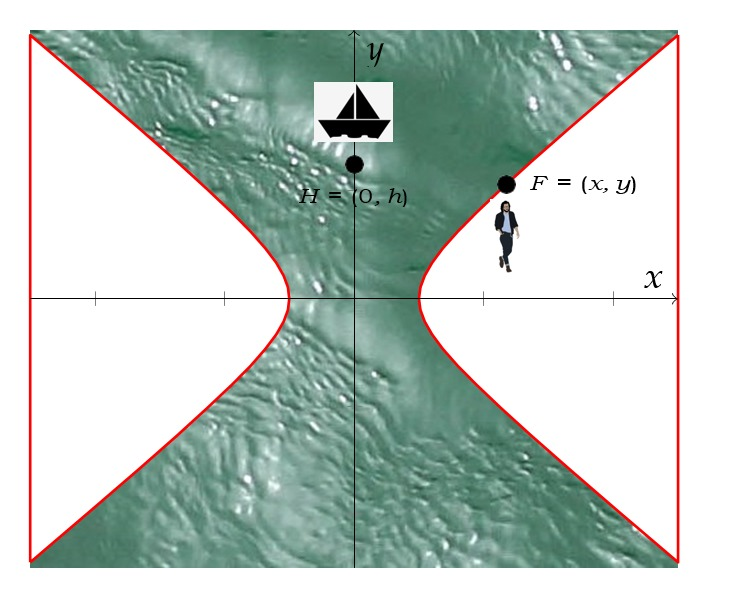
\includegraphics[width=0.7\textwidth]{pictures/1_c}
\end{center}
Der Fischer befindet sich an dem Punkt $ F= (x,y) $ am Flussufer.
Damit muss $ F = (x,y) $ die Hyperbelgleichung
\begin{align*}
	\frac{x^2}{a^2}- \frac{y^2}{b^2} = 1
\end{align*} 
erfüllen. Der Fischer möchte auf dem schnellsten Weg zu dem Punkt $ H = (0,h) $, d.h. wir wollen den Abstand von $ F  $ und $ H $ minimieren.
Es gilt
\begin{align*}
	| F - H |
	= 
	\sqrt{(x-0)^2 + (y-h)^2}
	=
	\underbrace{\sqrt{x^2 + (y-h)^2}}_{d(x,y) :=},
\end{align*}
wobei wir $ d $ als Abstandsfunktion bezeichnen.
Da die Wurzelfunktion streng monoton ist, können wir auch die einfachere Funktion 
\begin{align*}
	f(x,y) := x^2 + (y-h)^2 
\end{align*}
minimieren. Damit suchen wir
\begin{align*}
	\min \limits_{x,y} f(x,y) , \ \textrm{mit} \ \varphi(x,y) = \frac{x^2}{a^2} -\frac{y^2}{b^2} -1.
\end{align*}
\ \\
\underline{2. Wende die Lagrange-Methode an}\\
Zuerst stellen wir die Lagrange-Funktion auf:
\begin{align*}
	L(x,y, \lambda )
	= 
	f(x,y) + \lambda\cdot \varphi(x,y)
	=
	x^2 + (y-h)^2 + \lambda \cdot
	\left(\frac{x^2}{a^2} - \frac{y^2}{b^2} -1\right).
\end{align*}
Die partiellen Ableitungen sind:
\begin{align*}
	\frac{\partial L}{\partial x} (x,y,\lambda)
	&=
	2x + \frac{2 \lambda}{a^2} x\\
	\frac{\partial L}{\partial y} (x,y,\lambda)
	&=
	2(y-h)- \frac{2 \lambda}{b^2} y\\
	\frac{\partial L}{\partial\lambda} (x,y,\lambda)
	&=
	\frac{x^2}{a^2} - \frac{y^2}{b^2} -1.
\end{align*}
Durch Nullsetzen erhalten wir die Lagrange-Bedingungen:
\begin{align*}
	\textrm{(I)} &\ 2x + \frac{2 \lambda}{a^2} x = 0 \\
	\textrm{(II)} &\ 2(y-h)- \frac{2 \lambda}{b^2} y = 0\\
	\textrm{(III)} &\ \frac{x^2}{a^2} - \frac{y^2}{b^2} -1 = 0.
\end{align*}
Wir können $ x = 0 $ ausschließen, da ansonsten (III) verletzt wird. Damit gilt:
\begin{align*}
	\textrm{(I)}
	\ \Leftrightarrow \
	1 + \frac{\lambda}{a^2} = 0
	\ \Leftrightarrow \
	\frac{\lambda}{a^2} = - 1
	\ \Leftrightarrow \
	\lambda = - a^2.
\end{align*}
Einsetzen in (II) liefert:
\begin{align*}
	2 (y-h ) - \frac{2\lambda}{b^2} y
	&=
	2(y-h) +
	\frac{2 a^2}{b^2} y
	=2 y - 2h  + \frac{2 a^2}{b^2} y
	=
	2 \cdot \left(1 +   \frac{a^2}{b^2} \right) y - 2h 
	 = 0 \\
	\ \Leftrightarrow \
	\left(1 +   \frac{a^2}{b^2} \right) y  &= h
	\ \Leftrightarrow \
	y = \frac{h}{1 +   \frac{a^2}{b^2} }
	=
	\frac{h b^2 }{a^2 + b^2} \quad \textrm{(IV)}.
\end{align*}
Für die dritte Gleichung gilt:
\begin{align*}
	\textrm{(III)}
	\ \Leftrightarrow \
	\frac{x^2}{a^2} = 1+  \frac{y^2}{b^2} 
	\ \Leftrightarrow \
	x^2 = a^2 + \frac{a^2 y^2 }{b^2}
	\ \Leftrightarrow \
	x = \pm \sqrt{a^2 + \frac{a^2 y^2 }{b^2}}
	=
	\pm |a|  \sqrt{1 + \frac{y^2}{b^2}} \quad \textrm{(V)}
	.
\end{align*}
Zum Abschluss setzen wir (IV) in (V) ein:
\begin{align*}
	x =
	\pm |a|
	\sqrt{1 + \frac{\left(\frac{h b^2 }{a^2 + b^2}\right)^2}{b^2}} 
	=
	\pm |a| 
	\sqrt{1 + \frac{h^2 b^4}{(a^2 + b^2)^2} \cdot \frac{1 }{b^2}}
	=
	\pm |a| 
	\sqrt{1 + \frac{h^2 b^2}{(a^2 + b^2)^2}}.
\end{align*}
Damit haben wir zwei Punkte am Flussufer gefunden, welche den geringsten Abstand zu $ H $ besitzen.
Da die Hyperbel symmetrisch bezüglich der $ y $-Achse ist, sind die Punkte symmetrisch.
Die Stellen sind konkret:
\begin{align*}
	F_1 &=
	\left(|a| 
	\sqrt{1 + \frac{h^2 b^2}{(a^2 + b^2)^2}},\frac{h b^2 }{a^2 + b^2}  \right)\\
	F_2 &=
	\left(-|a| 
	\sqrt{1 + \frac{h^2 b^2}{(a^2 + b^2)^2}},\frac{h b^2 }{a^2 + b^2}  \right).
\end{align*}

\newpage
\subsection*{\aufgabe{d}{6}}
Die private Altersvorsorge gewinnt durch das Altern der Bevölkerung mehr und mehr an Bedeutung. Eine neue Gesetzesinitiative soll Anreize für eine Änderung des Sparverhaltens schaffen. Der (stochastische) Einfluss der Initiative auf den jährlichen Sparbetrag eines durchschnittlichen Haushalts soll nun modelliert werden. Es wird unterstellt, dass diese Änderung des Sparbetrags durch eine stetige Zufallsvariable $ D $ mit $ U $-quadratischer Verteilung modelliert werden kann.
Die Dichte von $ D $ sei gegeben durch:
\begin{align*}
	f(x)
	=
	\begin{cases}
		\frac{12}{(b-a)^3} \left(x - \frac{b+a}{2}\right)^2 \ &\textrm{für } x \in [a,b]\\ 
		\qquad \quad 0  \ &\quad \  \textrm{sonst}
	\end{cases},
\end{align*}
wobei $ a,b \in \mathbb{R} $, $ a < b $.
\begin{enumerate}
	\item[\textbf{(d1)}]
	Berechnen Sie für $ a = - 500 $ und $ b = 1000 $ die Wahrscheinlichkeit, dass der Sparbetrag eines durchschnittlichen Haushalts um mindestens CHF $ 200 $ erhöht wird.
	\item[\textbf{(d2)}]
	Berechnen Sie für $ a = - 500 $ und $ b = 1000 $ den erwarteten Anstieg des (durchschnittlichen) Sparbetrags $ \mathbb{E}[D] $.
\end{enumerate}

\textbf{Lösung:}
\begin{mdframed}
\underline{\textbf{Vorgehensweise:}}
\begin{enumerate}
\item[\textbf{(d1)}]
\begin{enumerate}
	\item[1.] Berechne die Wahrscheinlichkeit.
\end{enumerate}
\item[\textbf{(d2)}]
\begin{enumerate}
	\item[2.] Berechne den Erwartungswert.
\end{enumerate}
\end{enumerate}
\end{mdframed}

\underline{\textbf{(d1)} 1. Berechne die Wahrscheinlichkeit}\\
Wir sind an der Wahrscheinlichkeit interessiert, dass der Sparbetrag eines durchschnittlichen Haushalts um mindestens $ 200 $ (CHF) erhöht wird. 
Die Zufallsvariable $ D $ mit $ U $-quadratischer Verteilung modelliert die Änderung des Sparbetrags.
Damit erhalten wir durch 
\begin{align*}
	\mathbb{P}[D=\textrm{A}]
\end{align*}
die Wahrscheinlichkeit, dass ein durchschnittlicher Haushalt seinen Sparbetrag um den Betrag $ A $ erhöht.
Mit $ \mathbb{P}[D\geq \textrm{A}] $ drücken wir die Wahrscheinlichkeit aus, dass der Sparbetrag um mindestens $ A $ erhöht wird.
In der Aufgabenstellung ist $ a = -500  $ und $ b = 1000 $ gegeben. Wir werden die gesuchte Wahrscheinlichkeit jedoch für allgemeine $ a \leq b $ berechnen.
Es gilt:
\begin{align*}
	\mathbb{P}[D \geq 200 ]
	&=
	\int \limits_{200}^\infty f(x) \td{x}
	=
	\int \limits_{200}^b f(x) \td{x}
	=
	\int \limits_{200}^b 	\frac{12}{(b-a)^3} \left(x - \frac{b+a}{2}\right)^2\td{x}\\
	&=
	\frac{12}{(b-a)^3}\cdot \int \limits_{200}^b  \left(x - \frac{b+a}{2}\right)^2\td{x}
	=
	\frac{12}{(b-a)^3}\cdot
	\left[
	\frac{1}{3}\left(x - \frac{b + a }{2}\right)^3
	\right]_{200}^b\\
	&=
	\frac{12}{(b-a)^3}\cdot \frac{1}{3} \cdot
	\left(
	\left(b - \frac{b + a }{2}\right)^3
	-
	\left(200- \frac{b + a }{2}\right)^3
	\right)\\
	&=
	\frac{4}{(b-a)^3} \cdot
	\left(
	\left(\frac{2b}{2} - \frac{b + a }{2}\right)^3
	-
	\left(200- \frac{b + a }{2}\right)^3
	\right)\\
	&=
	\frac{4}{(b-a)^3} \cdot
	\left(
	\left( \frac{b - a }{2}\right)^3
	-
	\left(200- \frac{b + a }{2}\right)^3
	\right)\\
	&=
	\frac{4}{(b-a)^3} \cdot \frac{(b-a)^3 }{2^3}
	- 
	\frac{4}{(b-a)^3} \cdot \left(200- \frac{b + a }{2}\right)^3
	=
	\frac{1}{2}
	- 
	\frac{4}{(b-a)^3} \cdot \left(200- \frac{b + a }{2}\right)^3\\
	&=
	\frac{1}{2}
	- 
	4 \cdot \left(\frac{200}{b-a}- \frac{b + a }{2(b-a)}\right)^3.
\end{align*}
Nun können wir die Werte $ a = -500  $ und $ b = 1000 $ einfügen. Damit erhalten wir:
\begin{align*}
	\mathbb{P}[D \geq 200 ]
	&=
	\frac{1}{2}
	- 
	4 \cdot \left(\frac{200}{1500}- \frac{500 }{2\cdot 1500}\right)^3
	=
	\frac{1}{2}
	- 
	4 \cdot \left(\frac{2}{15}- \frac{1 }{2\cdot 3}\right)^3
	=
	\frac{1}{2}
	- 
	4 \cdot \left(\frac{2}{15}- \frac{1 }{6}\right)^3\\
	&=
	\frac{1}{2}
	- 
	4 \cdot \left(\frac{8}{60}- \frac{10 }{60}\right)^3
	=
	\frac{1}{2}
	- 
	4 \cdot \left(\frac{-2}{60}\right)^3
	=
	\frac{1}{2}
	- 
	4 \cdot \frac{-8}{60^3}
	=
	\frac{1}{2}
	+
	\frac{32}{60^3}\\
	&\approx
	0.5001481.
\end{align*}
Damit beträgt die Wahrscheinlichkeit, dass der Sparbetrag um mindestens $ 200 $ (CHF) erhöht wird ungefähr $ 50.01 \% $.\\
\\
\underline{\textbf{(d2)} 1. Berechne den Erwartungswert}\\
Der erwartete Anstieg des durchschnittlichen Sparbetrags ergibt sich durch:
\begin{align*}
	\mathbb{E}[D]
	&=
	\int \limits_{-\infty}^\infty x f(x) \td{x}
	=
	\int \limits_a^b
	x  \frac{12}{(b-a)^3} \left(x - \frac{b+a}{2}\right)^2
	\td{x}
	=
	\frac{12}{(b-a)^3}
	\int \limits_a^b
	x   \left(x^2 - (b-a) x + \frac{(b+a)^2}{4}\right)
	\td{x}\\
	&=
	\frac{12}{(b-a)^3}
	\int \limits_a^b
	x^3 - (b-a) x^2 + \frac{(b+a)^2}{4} x \
	\td{x}
	=
	\frac{12}{(b-a)^3}
	\left[
	\frac{1}{4} x^4 - \frac{b+a}{3} x^3 + \frac{(b+a)^2}{8} x^2 
	\right]_a^b\\
	&=
	\frac{12}{(b-a)^3}
	\left(
	\frac{b^4}{4} - \frac{b+a}{3} \cdot b^3 + \frac{(b+a)^2}{8}\cdot  b^2
	- 
	\frac{a^4}{4} + \frac{b+a}{3} \cdot a^3 -\frac{(b+a)^2}{8} \cdot a^2
	\right)\\
	&=
	\frac{12}{(b-a)^3}
	\left(
	\frac{b^4 - a^4}{4} - \frac{b+a}{3} (b^3 - a^3) + \frac{(b+a)^2}{8} (b^2 -a^2)
	\right)\\
	&=
	\frac{12}{(b-a)^3}
	\left(
	\frac{(b^2 + a^2) (b^2- a^2)}{4} - \frac{b+a}{3} (b^3 - a^3) + \frac{(b+a)^2}{8} (b^2 -a^2)
	\right)\\
	&=
	\frac{12}{(b-a)^3}
	\left(
	\frac{1}{2}(b^2- a^2) \left(\frac{ b^2 + a^2 }{2} + \frac{(b+a)^2}{4}\right)  - \frac{b+a}{3} (b^3 - a^3) 
	\right)\\
	&=
	\frac{12}{(b-a)^3}
	\left(
	\frac{1}{2}(b^2- a^2) \left(\frac{ 2b^2 + 2a^2 }{4} + \frac{a^2 + 2 ab +b^2}{4}\right)  - \frac{b+a}{3} (b^3 - a^3) 
	\right)\\
	&=
	\frac{12}{(b-a)^3}
	\left(
	\frac{1}{8}(b^2- a^2) \left(3a^2 + 2ab +3 b^2\right)  - \frac{b+a}{3} (b^3 - a^3) 
	\right)\\
	&=
	\frac{12}{(b-a)^3}
	\left(
	\frac{1}{8}(b^2- a^2) \left(3a^2 + 2ab +3 b^2\right)  - \frac{1}{3} (b^4  - a^3b + a b^3 - a^4) 
	\right)\\
	&=
	\frac{12}{(b-a)^3}
	\left(
	\frac{1}{8} \left(3a^2 b^2 + 2ab^3 +3 b^4
	-3 a^4 -2a^3 b -3a^2 b^2
	\right)  - \frac{1}{3} (b^4  - a^3b + a b^3 - a^4) 
	\right)\\
	&=
	\frac{12}{(b-a)^3}
	\left(
	\frac{1}{8} \left(3 b^4 +2ab^3 
	 -2a^3 b -3 a^4 
	\right)  - \frac{1}{3} (b^4  - a^3b + a b^3 - a^4) 
	\right)\\
	&=
	\frac{12}{(b-a)^3}
	\left(
	\frac{3}{24} \left(3 b^4 +2ab^3 
	-2a^3 b -3 a^4 
	\right)  - \frac{8}{24} (b^4  - a^3b + a b^3 - a^4) 
	\right)\\
	&=
	\frac{1}{(b-a)^3} \frac{1}{2}
	\left(
	3 \cdot \left(3 b^4 +2ab^3 
	-2a^3 b -3 a^4 
	\right)  - 8 \cdot (b^4  - a^3b + a b^3 - a^4) 
	\right)\\
	&=
	\frac{1}{(b-a)^3} \frac{1}{2}
	\left(
	9 b^4 +6ab^3 
	-6a^3 b -9 a^4 
	  - 8 b^4  +8 a^3b - 8 a b^3 + 8 a^4) 
	\right)\\
	&=
	\frac{1}{(b-a)^3} \frac{1}{2}
	\left(
	  b^4 
	  +2a^3 b
	  -2ab^3  
	- a^4  
	\right)\\
	&=
	\frac{1}{(b-a)^3} \frac{1}{2}
	\left(
	b-a  
	\right)^3 (b+a)\\
	&=
	\frac{b+a}{2}.
\end{align*}
Da die Dichtefunktion symmetrisch bezüglich $ \frac{b+a}{2} $ ist, kann man auch direkt sagen, dass $ \mathbb{E}[D]= \frac{b+a}{2} $ gilt.
Dies ist möglich, da $ \frac{a+b}{2} $ der Mittelwert auf dem Intervall $ [a,b] $ ist.
Mit $ a= -500 $ und $ b = 1000 $ erhalten wir:
\begin{align*}
	\mathbb{E}[D]
	=
	\frac{1000 - 500}{2}
	=
	\frac{500}{2}
	=
	250.
\end{align*}
Damit beträgt der erwartete Anstieg der durchschnittlichen Sparrate $ 250 $.
\newpage

